\begin{frame}[fragile]{Visualização do algoritmo de Morris-Pratt}

    \begin{figure}
        \centering

        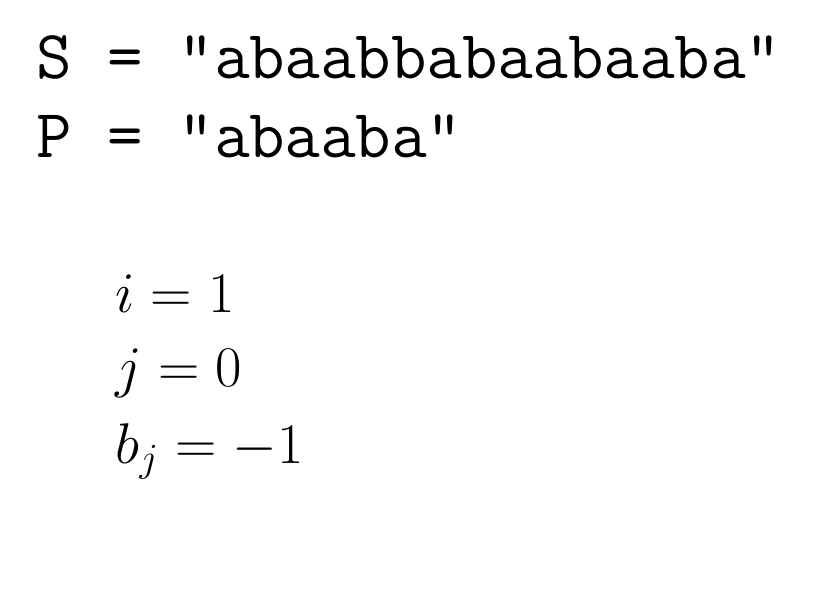
\begin{tikzpicture}
            \node[anchor=west] at (6, 5) { \Huge \texttt{S = "\textcolor{blue}{}abaabbabaabaaba"} };
            \node[anchor=west] at (6, 4) { \Huge \texttt{P = "\textcolor{blue}{}abaaba"} };

            \node[anchor=west] at (7, 2) { \huge $i = 1$ };
            \node[anchor=west] at (7, 1) { \huge $j = 0$ };
            \node[anchor=west] at (7, 0) { \huge $b_j = -1$ };
            \node[opacity=0,anchor=west] at (7, -1) { \huge $s = -1$ };
        \end{tikzpicture}

    \end{figure}

\end{frame}

\begin{frame}[fragile]{Visualização do algoritmo de Morris-Pratt}

    \begin{figure}
        \centering

        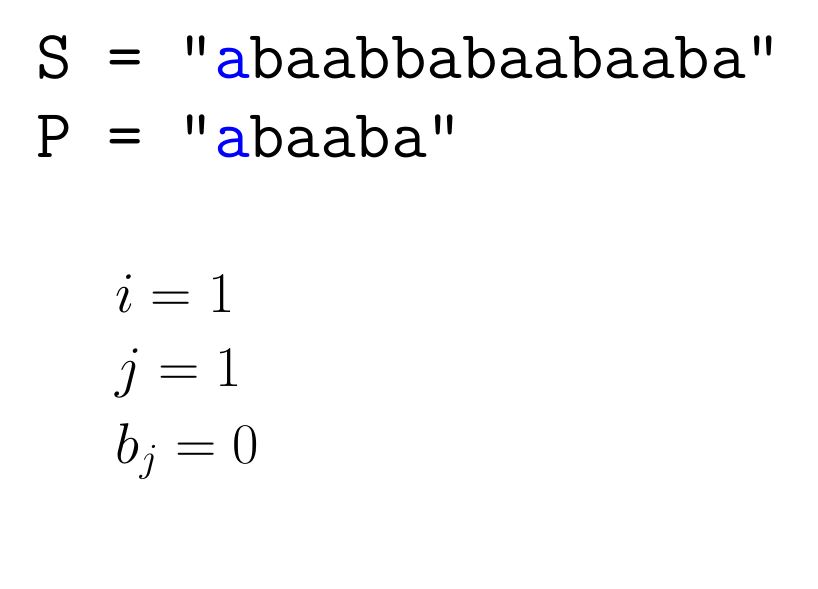
\begin{tikzpicture}
            \node[anchor=west] at (6, 5) { \Huge \texttt{S = "\textcolor{blue}{a}baabbabaabaaba"} };
            \node[anchor=west] at (6, 4) { \Huge \texttt{P = "\textcolor{blue}{a}baaba"} };

            \node[anchor=west] at (7, 2) { \huge $i = 1$ };
            \node[anchor=west] at (7, 1) { \huge $j = 1$ };
            \node[anchor=west] at (7, 0) { \huge $b_j = 0$ };
            \node[opacity=0,anchor=west] at (7, -1) { \huge $s = -1$ };
        \end{tikzpicture}

    \end{figure}

\end{frame}

\begin{frame}[fragile]{Visualização do algoritmo de Morris-Pratt}

    \begin{figure}
        \centering

        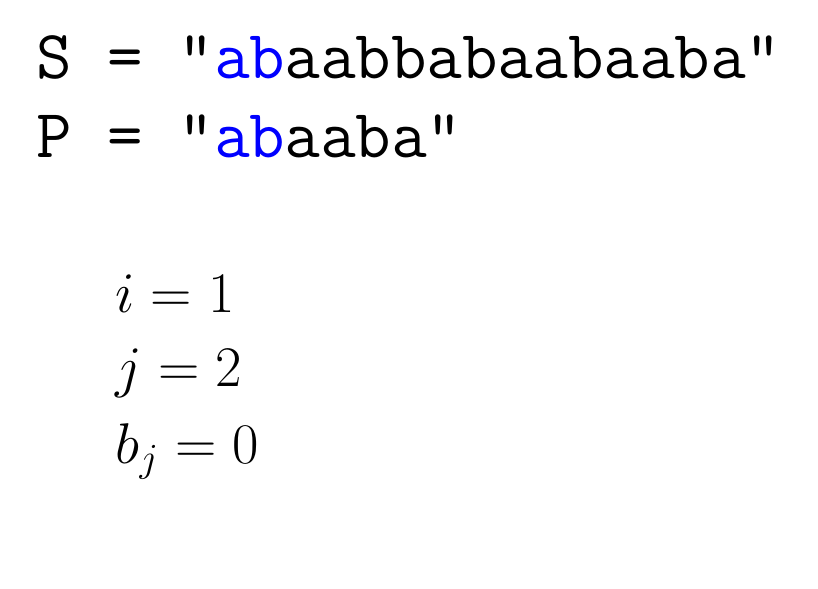
\begin{tikzpicture}
            \node[anchor=west] at (6, 5) { \Huge \texttt{S = "\textcolor{blue}{ab}aabbabaabaaba"} };
            \node[anchor=west] at (6, 4) { \Huge \texttt{P = "\textcolor{blue}{ab}aaba"} };

            \node[anchor=west] at (7, 2) { \huge $i = 1$ };
            \node[anchor=west] at (7, 1) { \huge $j = 2$ };
            \node[anchor=west] at (7, 0) { \huge $b_j = 0$ };
            \node[opacity=0,anchor=west] at (7, -1) { \huge $s = -1$ };
        \end{tikzpicture}

    \end{figure}

\end{frame}

\begin{frame}[fragile]{Visualização do algoritmo de Morris-Pratt}

    \begin{figure}
        \centering

        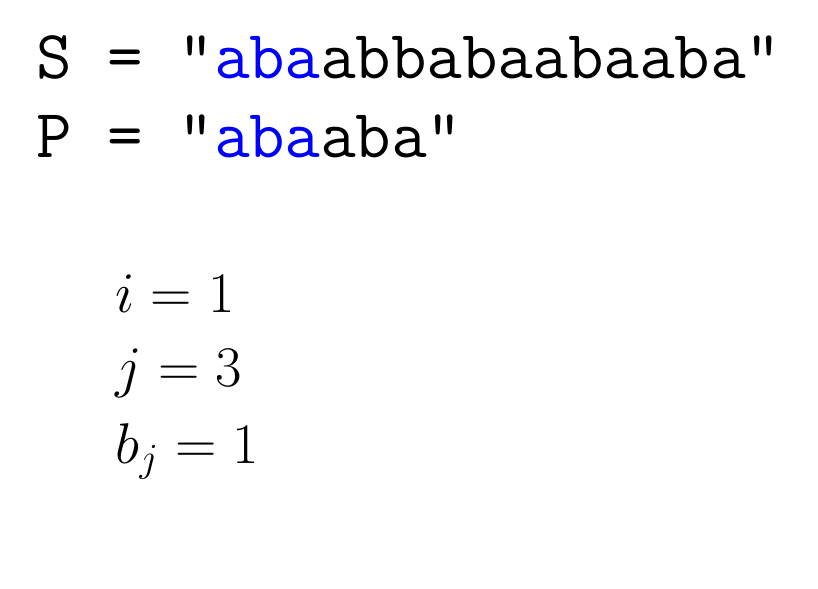
\begin{tikzpicture}
            \node[anchor=west] at (6, 5) { \Huge \texttt{S = "\textcolor{blue}{aba}abbabaabaaba"} };
            \node[anchor=west] at (6, 4) { \Huge \texttt{P = "\textcolor{blue}{aba}aba"} };

            \node[anchor=west] at (7, 2) { \huge $i = 1$ };
            \node[anchor=west] at (7, 1) { \huge $j = 3$ };
            \node[anchor=west] at (7, 0) { \huge $b_j = 1$ };
            \node[opacity=0,anchor=west] at (7, -1) { \huge $s = -1$ };
        \end{tikzpicture}

    \end{figure}

\end{frame}

\begin{frame}[fragile]{Visualização do algoritmo de Morris-Pratt}

    \begin{figure}
        \centering

        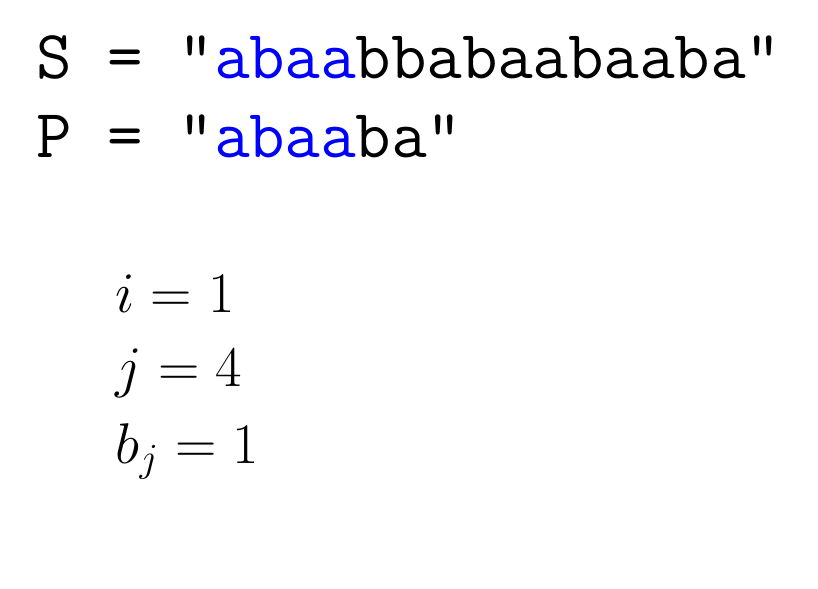
\begin{tikzpicture}
            \node[anchor=west] at (6, 5) { \Huge \texttt{S = "\textcolor{blue}{abaa}bbabaabaaba"} };
            \node[anchor=west] at (6, 4) { \Huge \texttt{P = "\textcolor{blue}{abaa}ba"} };

            \node[anchor=west] at (7, 2) { \huge $i = 1$ };
            \node[anchor=west] at (7, 1) { \huge $j = 4$ };
            \node[anchor=west] at (7, 0) { \huge $b_j = 1$ };
            \node[opacity=0,anchor=west] at (7, -1) { \huge $s = -1$ };
        \end{tikzpicture}

    \end{figure}

\end{frame}

\begin{frame}[fragile]{Visualização do algoritmo de Morris-Pratt}

    \begin{figure}
        \centering

        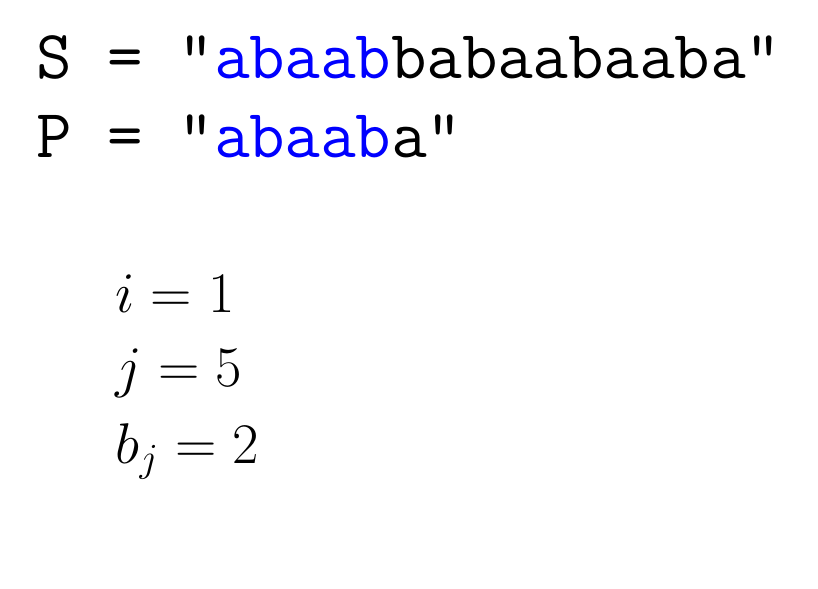
\begin{tikzpicture}
            \node[anchor=west] at (6, 5) { \Huge \texttt{S = "\textcolor{blue}{abaab}babaabaaba"} };
            \node[anchor=west] at (6, 4) { \Huge \texttt{P = "\textcolor{blue}{abaab}a"} };

            \node[anchor=west] at (7, 2) { \huge $i = 1$ };
            \node[anchor=west] at (7, 1) { \huge $j = 5$ };
            \node[anchor=west] at (7, 0) { \huge $b_j = 2$ };
            \node[opacity=0,anchor=west] at (7, -1) { \huge $s = -1$ };
        \end{tikzpicture}

    \end{figure}

\end{frame}

\begin{frame}[fragile]{Visualização do algoritmo de Morris-Pratt}

    \begin{figure}
        \centering

        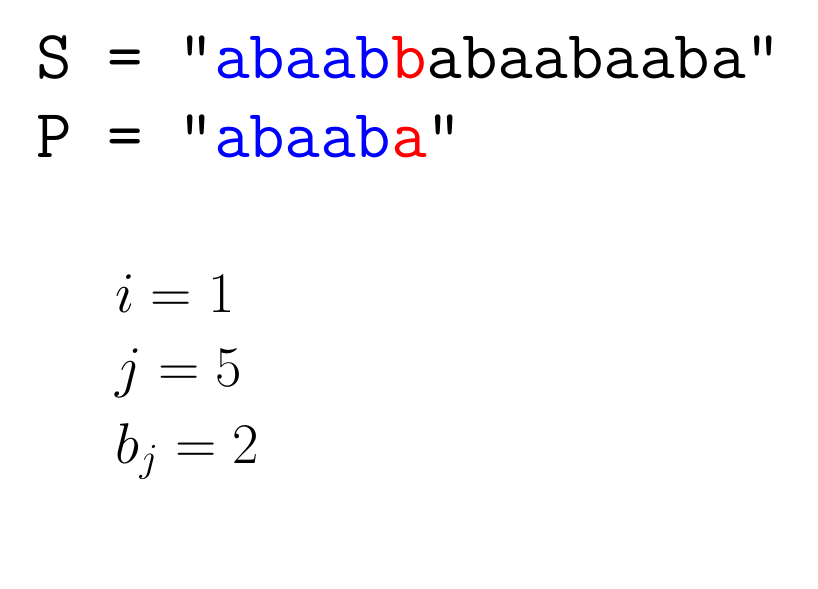
\begin{tikzpicture}
            \node[anchor=west] at (6, 5) { \Huge \texttt{S = "\textcolor{blue}{abaab}\textcolor{red}{b}abaabaaba"} };
            \node[anchor=west] at (6, 4) { \Huge \texttt{P = "\textcolor{blue}{abaab}\textcolor{red}{a}"} };

            \node[anchor=west] at (7, 2) { \huge $i = 1$ };
            \node[anchor=west] at (7, 1) { \huge $j = 5$ };
            \node[anchor=west] at (7, 0) { \huge $b_j = 2$ };
            \node[opacity=0,anchor=west] at (7, -1) { \huge $s = -1$ };
        \end{tikzpicture}

    \end{figure}

\end{frame}

\begin{frame}[fragile]{Visualização do algoritmo de Morris-Pratt}

    \begin{figure}
        \centering

        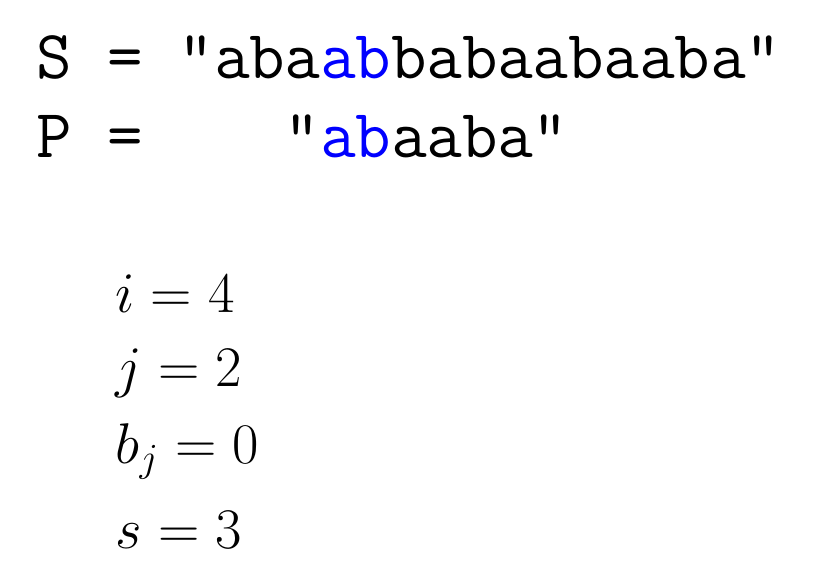
\begin{tikzpicture}
            \node[anchor=west] at (6, 5) { \Huge \texttt{S = "aba\textcolor{blue}{ab}\textcolor{red}{}babaabaaba"} };
            \node[anchor=west] at (6, 4) { \Huge \texttt{P = \ \ \ "\textcolor{blue}{ab}aaba"} };

            \node[anchor=west] at (7, 2) { \huge $i = 4$ };
            \node[anchor=west] at (7, 1) { \huge $j = 2$ };
            \node[anchor=west] at (7, 0) { \huge $b_j = 0$ };
            \node[opacity=1,anchor=west] at (7, -1) { \huge $s = 3$ };
        \end{tikzpicture}

    \end{figure}

\end{frame}

\begin{frame}[fragile]{Visualização do algoritmo de Morris-Pratt}

    \begin{figure}
        \centering

        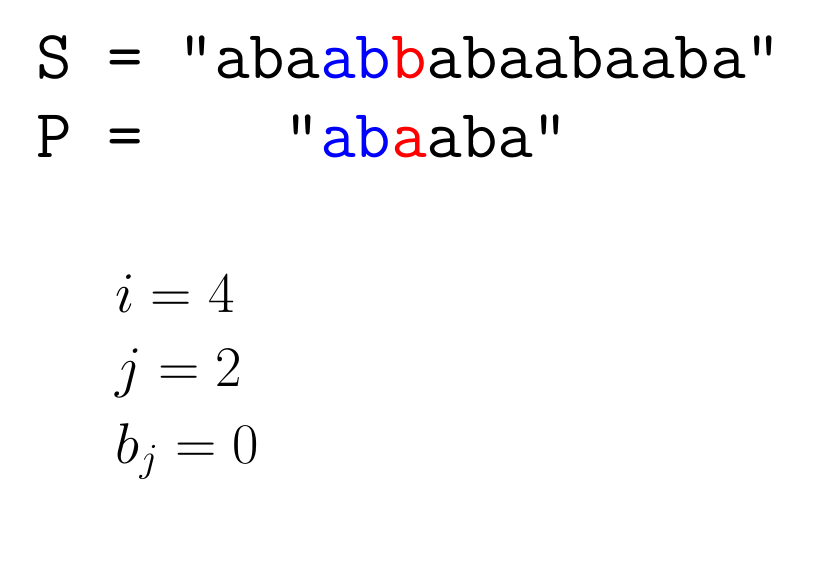
\begin{tikzpicture}
            \node[anchor=west] at (6, 5) { \Huge \texttt{S = "aba\textcolor{blue}{ab}\textcolor{red}{b}abaabaaba"} };
            \node[anchor=west] at (6, 4) { \Huge \texttt{P = \ \ \ "\textcolor{blue}{ab}\textcolor{red}{a}aba"} };

            \node[anchor=west] at (7, 2) { \huge $i = 4$ };
            \node[anchor=west] at (7, 1) { \huge $j = 2$ };
            \node[anchor=west] at (7, 0) { \huge $b_j = 0$ };
            \node[opacity=0,anchor=west] at (7, -1) { \huge $s = 3$ };
        \end{tikzpicture}

    \end{figure}

\end{frame}

\begin{frame}[fragile]{Visualização do algoritmo de Morris-Pratt}

    \begin{figure}
        \centering

        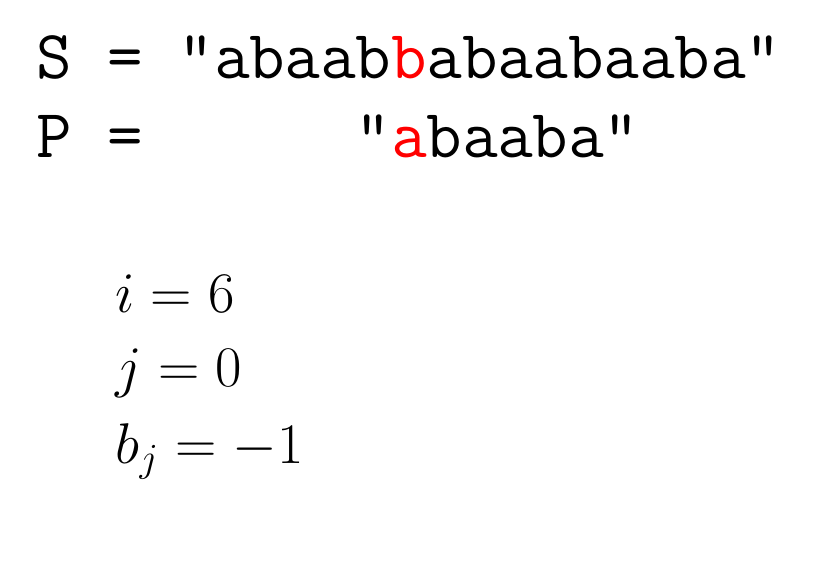
\begin{tikzpicture}
            \node[anchor=west] at (6, 5) { \Huge \texttt{S = "abaab\textcolor{blue}{}\textcolor{red}{b}abaabaaba"} };
            \node[anchor=west] at (6, 4) { \Huge \texttt{P = \ \ \ \ \ "\textcolor{blue}{}\textcolor{red}{a}baaba"} };

            \node[anchor=west] at (7, 2) { \huge $i = 6$ };
            \node[anchor=west] at (7, 1) { \huge $j = 0$ };
            \node[anchor=west] at (7, 0) { \huge $b_j = -1$ };
            \node[opacity=0,anchor=west] at (7, -1) { \huge $s = 2$ };
        \end{tikzpicture}

    \end{figure}

\end{frame}

\begin{frame}[fragile]{Visualização do algoritmo de Morris-Pratt}

    \begin{figure}
        \centering

        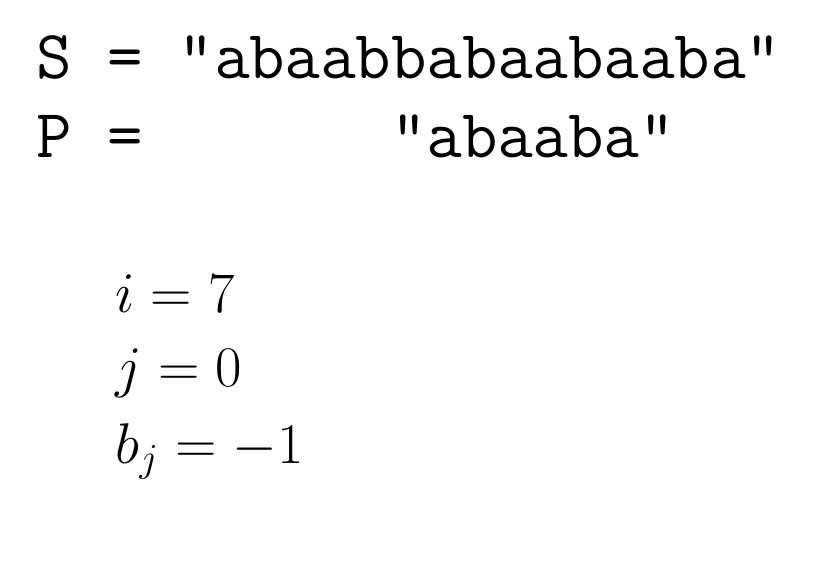
\begin{tikzpicture}
            \node[anchor=west] at (6, 5) { \Huge \texttt{S = "abaabb\textcolor{blue}{}\textcolor{red}{}abaabaaba"} };
            \node[anchor=west] at (6, 4) { \Huge \texttt{P = \ \ \ \ \ \ "\textcolor{blue}{}\textcolor{red}{}abaaba"} };

            \node[anchor=west] at (7, 2) { \huge $i = 7$ };
            \node[anchor=west] at (7, 1) { \huge $j = 0$ };
            \node[anchor=west] at (7, 0) { \huge $b_j = -1$ };
            \node[opacity=0,anchor=west] at (7, -1) { \huge $s = 1$ };
        \end{tikzpicture}

    \end{figure}

\end{frame}

\begin{frame}[fragile]{Visualização do algoritmo de Morris-Pratt}

    \begin{figure}
        \centering

        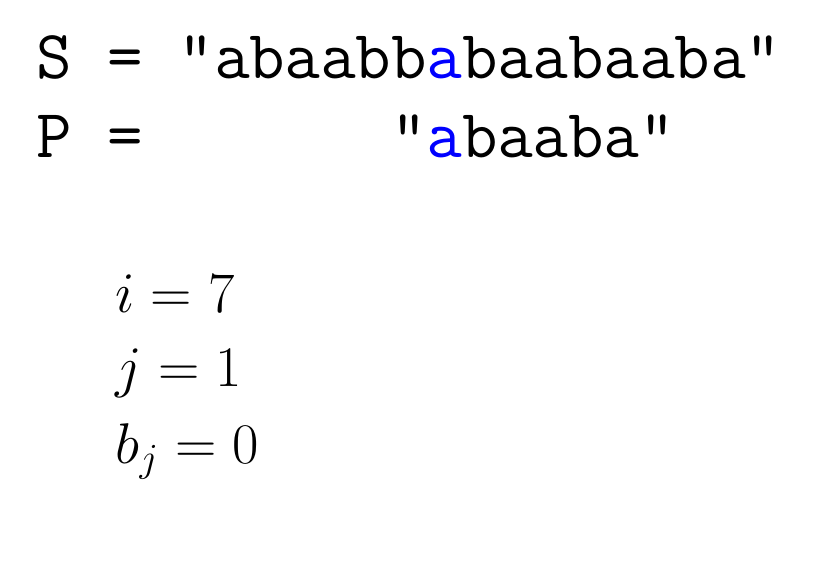
\begin{tikzpicture}
            \node[anchor=west] at (6, 5) { \Huge \texttt{S = "abaabb\textcolor{blue}{a}\textcolor{red}{}baabaaba"} };
            \node[anchor=west] at (6, 4) { \Huge \texttt{P = \ \ \ \ \ \ "\textcolor{blue}{a}\textcolor{red}{}baaba"} };

            \node[anchor=west] at (7, 2) { \huge $i = 7$ };
            \node[anchor=west] at (7, 1) { \huge $j = 1$ };
            \node[anchor=west] at (7, 0) { \huge $b_j = 0$ };
            \node[opacity=0,anchor=west] at (7, -1) { \huge $s = 1$ };
        \end{tikzpicture}

    \end{figure}

\end{frame}

\begin{frame}[fragile]{Visualização do algoritmo de Morris-Pratt}

    \begin{figure}
        \centering

        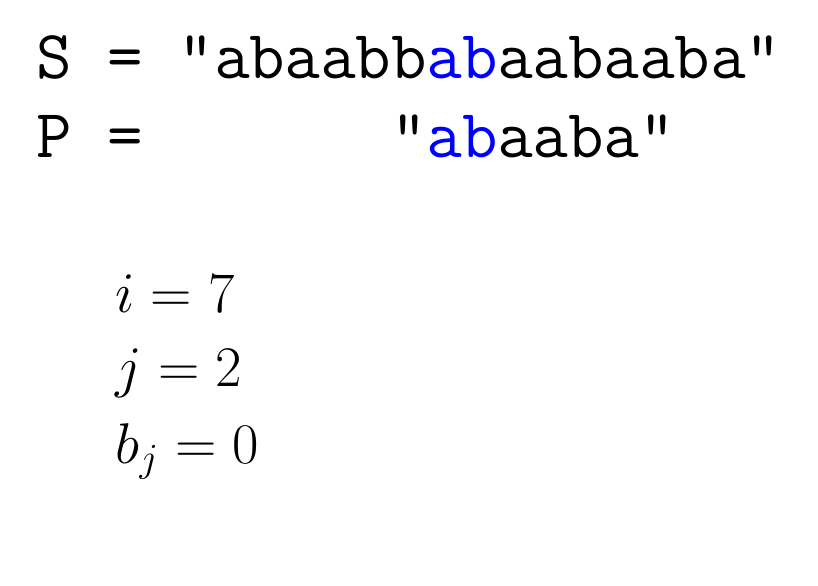
\begin{tikzpicture}
            \node[anchor=west] at (6, 5) { \Huge \texttt{S = "abaabb\textcolor{blue}{ab}\textcolor{red}{}aabaaba"} };
            \node[anchor=west] at (6, 4) { \Huge \texttt{P = \ \ \ \ \ \ "\textcolor{blue}{ab}\textcolor{red}{}aaba"} };

            \node[anchor=west] at (7, 2) { \huge $i = 7$ };
            \node[anchor=west] at (7, 1) { \huge $j = 2$ };
            \node[anchor=west] at (7, 0) { \huge $b_j = 0$ };
            \node[opacity=0,anchor=west] at (7, -1) { \huge $s = 1$ };
        \end{tikzpicture}

    \end{figure}

\end{frame}

\begin{frame}[fragile]{Visualização do algoritmo de Morris-Pratt}

    \begin{figure}
        \centering

        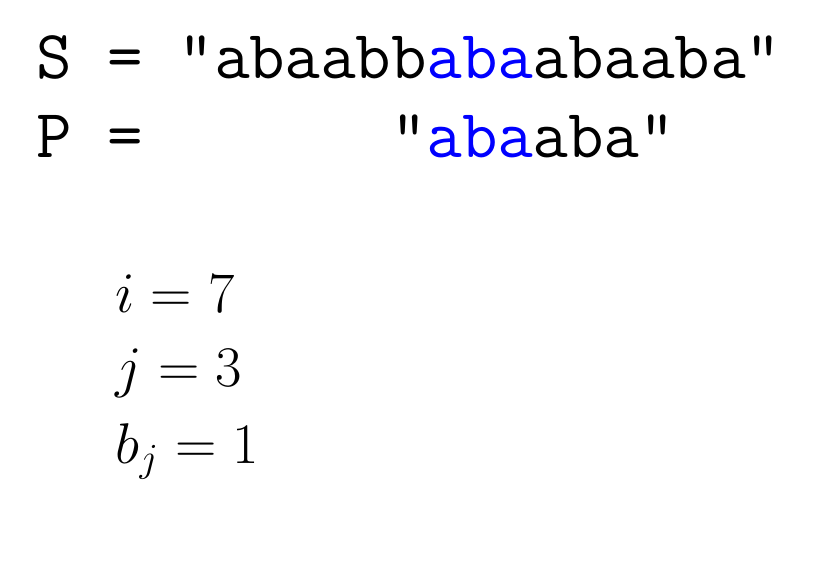
\begin{tikzpicture}
            \node[anchor=west] at (6, 5) { \Huge \texttt{S = "abaabb\textcolor{blue}{aba}\textcolor{red}{}abaaba"} };
            \node[anchor=west] at (6, 4) { \Huge \texttt{P = \ \ \ \ \ \ "\textcolor{blue}{aba}\textcolor{red}{}aba"} };

            \node[anchor=west] at (7, 2) { \huge $i = 7$ };
            \node[anchor=west] at (7, 1) { \huge $j = 3$ };
            \node[anchor=west] at (7, 0) { \huge $b_j = 1$ };
            \node[opacity=0,anchor=west] at (7, -1) { \huge $s = 1$ };
        \end{tikzpicture}

    \end{figure}

\end{frame}

\begin{frame}[fragile]{Visualização do algoritmo de Morris-Pratt}

    \begin{figure}
        \centering

        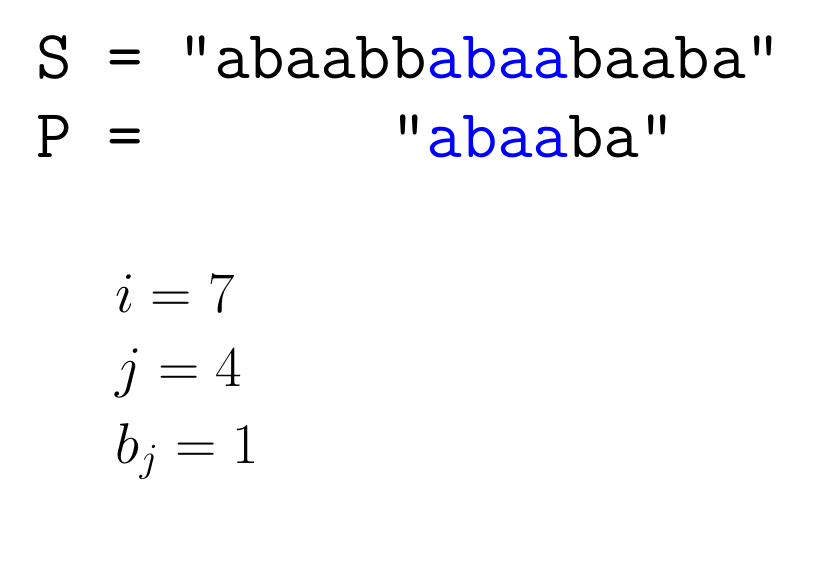
\begin{tikzpicture}
            \node[anchor=west] at (6, 5) { \Huge \texttt{S = "abaabb\textcolor{blue}{abaa}\textcolor{red}{}baaba"} };
            \node[anchor=west] at (6, 4) { \Huge \texttt{P = \ \ \ \ \ \ "\textcolor{blue}{abaa}\textcolor{red}{}ba"} };

            \node[anchor=west] at (7, 2) { \huge $i = 7$ };
            \node[anchor=west] at (7, 1) { \huge $j = 4$ };
            \node[anchor=west] at (7, 0) { \huge $b_j = 1$ };
            \node[opacity=0,anchor=west] at (7, -1) { \huge $s = 1$ };
        \end{tikzpicture}

    \end{figure}

\end{frame}

\begin{frame}[fragile]{Visualização do algoritmo de Morris-Pratt}

    \begin{figure}
        \centering

        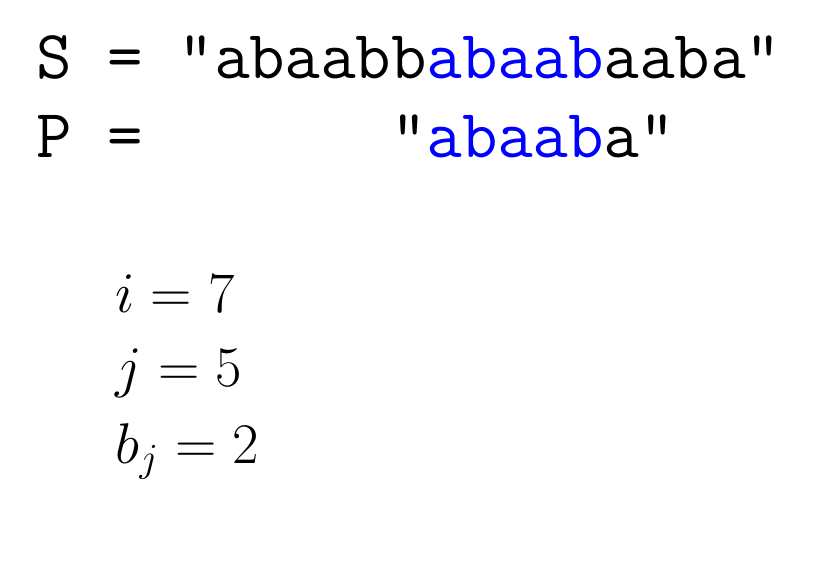
\begin{tikzpicture}
            \node[anchor=west] at (6, 5) { \Huge \texttt{S = "abaabb\textcolor{blue}{abaab}\textcolor{red}{}aaba"} };
            \node[anchor=west] at (6, 4) { \Huge \texttt{P = \ \ \ \ \ \ "\textcolor{blue}{abaab}\textcolor{red}{}a"} };

            \node[anchor=west] at (7, 2) { \huge $i = 7$ };
            \node[anchor=west] at (7, 1) { \huge $j = 5$ };
            \node[anchor=west] at (7, 0) { \huge $b_j = 2$ };
            \node[opacity=0,anchor=west] at (7, -1) { \huge $s = 1$ };
        \end{tikzpicture}

    \end{figure}

\end{frame}

\begin{frame}[fragile]{Visualização do algoritmo de Morris-Pratt}

    \begin{figure}
        \centering

        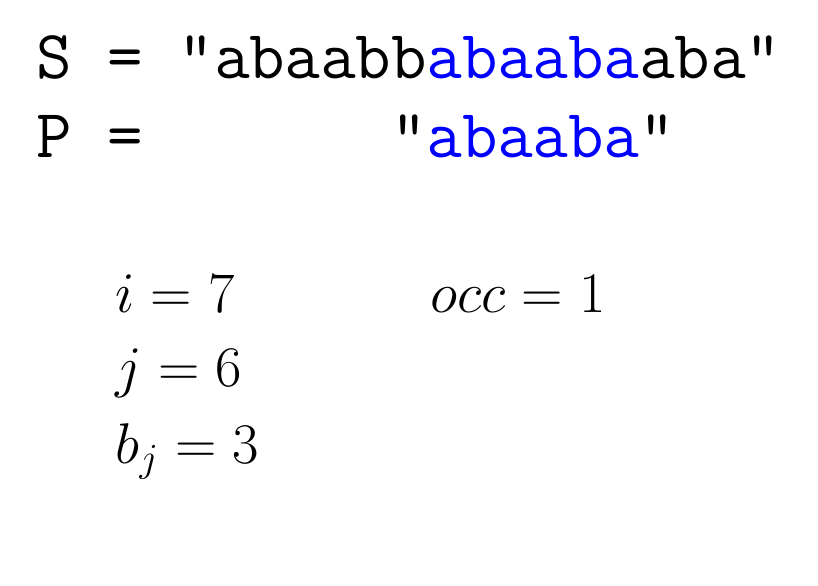
\begin{tikzpicture}
            \node[anchor=west] at (6, 5) { \Huge \texttt{S = "abaabb\textcolor{blue}{abaaba}\textcolor{red}{}aba"} };
            \node[anchor=west] at (6, 4) { \Huge \texttt{P = \ \ \ \ \ \ "\textcolor{blue}{abaaba}\textcolor{red}{}"} };

            \node[anchor=west] at (7, 2) { \huge $i = 7$ };
            \node[anchor=west] at (11, 2) { \huge $occ = 1$ };
            \node[anchor=west] at (7, 1) { \huge $j = 6$ };
            \node[anchor=west] at (7, 0) { \huge $b_j = 3$ };
            \node[opacity=0,anchor=west] at (7, -1) { \huge $s = 1$ };
        \end{tikzpicture}

    \end{figure}

\end{frame}

\begin{frame}[fragile]{Visualização do algoritmo de Morris-Pratt}

    \begin{figure}
        \centering

        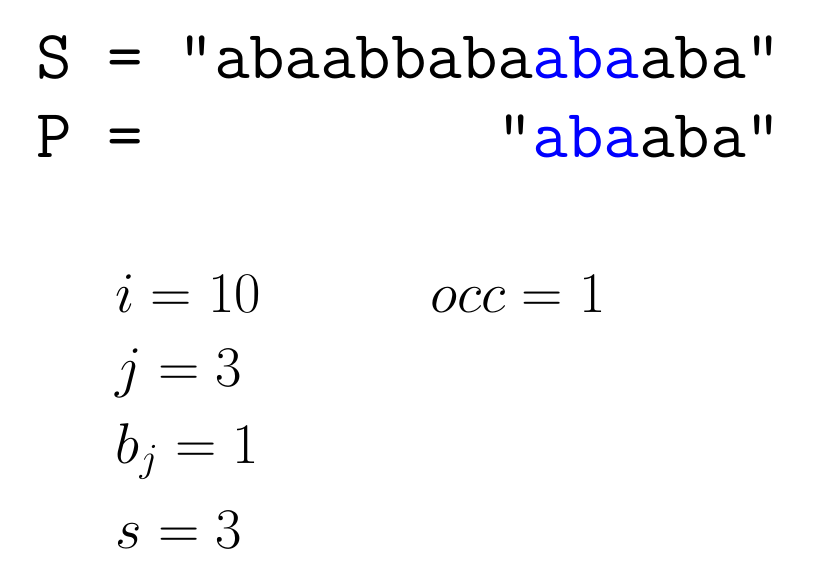
\begin{tikzpicture}
            \node[anchor=west] at (6, 5) { \Huge \texttt{S = "abaabbaba\textcolor{blue}{aba}\textcolor{red}{}aba"} };
            \node[anchor=west] at (6, 4) { \Huge \texttt{P = \ \ \ \ \ \ \ \ \ "\textcolor{blue}{aba}aba"} };

            \node[anchor=west] at (7, 2) { \huge $i = 10$ };
            \node[anchor=west] at (11, 2) { \huge $occ = 1$ };
            \node[anchor=west] at (7, 1) { \huge $j = 3$ };
            \node[anchor=west] at (7, 0) { \huge $b_j = 1$ };
            \node[opacity=1,anchor=west] at (7, -1) { \huge $s = 3$ };
        \end{tikzpicture}

    \end{figure}

\end{frame}

\begin{frame}[fragile]{Visualização do algoritmo de Morris-Pratt}

    \begin{figure}
        \centering

        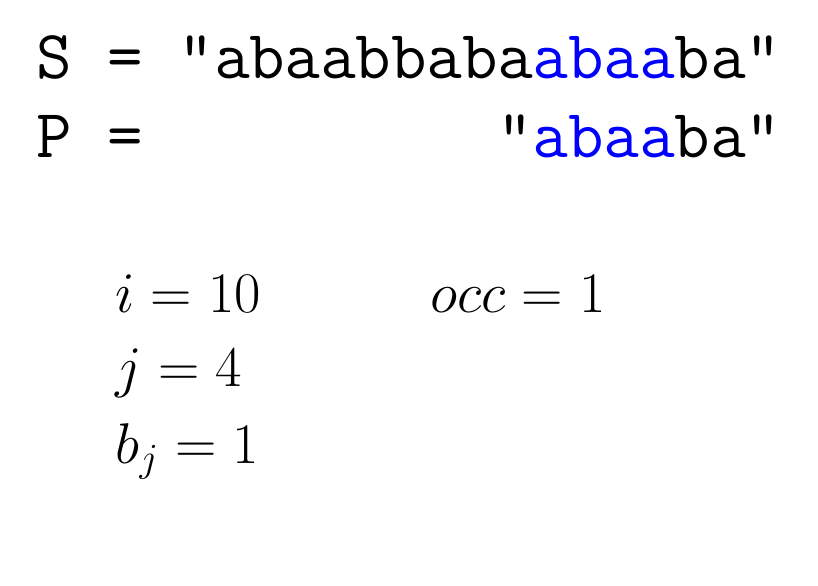
\begin{tikzpicture}
            \node[anchor=west] at (6, 5) { \Huge \texttt{S = "abaabbaba\textcolor{blue}{abaa}\textcolor{red}{}ba"} };
            \node[anchor=west] at (6, 4) { \Huge \texttt{P = \ \ \ \ \ \ \ \ \ "\textcolor{blue}{abaa}ba"} };

            \node[anchor=west] at (7, 2) { \huge $i = 10$ };
            \node[anchor=west] at (11, 2) { \huge $occ = 1$ };
            \node[anchor=west] at (7, 1) { \huge $j = 4$ };
            \node[anchor=west] at (7, 0) { \huge $b_j = 1$ };
            \node[opacity=0,anchor=west] at (7, -1) { \huge $s = 3$ };
        \end{tikzpicture}

    \end{figure}

\end{frame}

\begin{frame}[fragile]{Visualização do algoritmo de Morris-Pratt}

    \begin{figure}
        \centering

        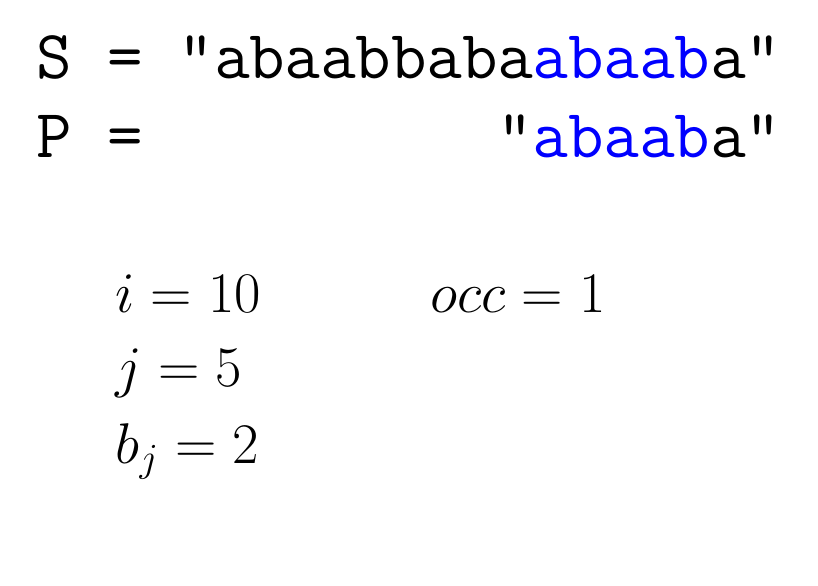
\begin{tikzpicture}
            \node[anchor=west] at (6, 5) { \Huge \texttt{S = "abaabbaba\textcolor{blue}{abaab}\textcolor{red}{}a"} };
            \node[anchor=west] at (6, 4) { \Huge \texttt{P = \ \ \ \ \ \ \ \ \ "\textcolor{blue}{abaab}a"} };

            \node[anchor=west] at (7, 2) { \huge $i = 10$ };
            \node[anchor=west] at (11, 2) { \huge $occ = 1$ };
            \node[anchor=west] at (7, 1) { \huge $j = 5$ };
            \node[anchor=west] at (7, 0) { \huge $b_j = 2$ };
            \node[opacity=0,anchor=west] at (7, -1) { \huge $s = 3$ };
        \end{tikzpicture}

    \end{figure}

\end{frame}

\begin{frame}[fragile]{Visualização do algoritmo de Morris-Pratt}

    \begin{figure}
        \centering

        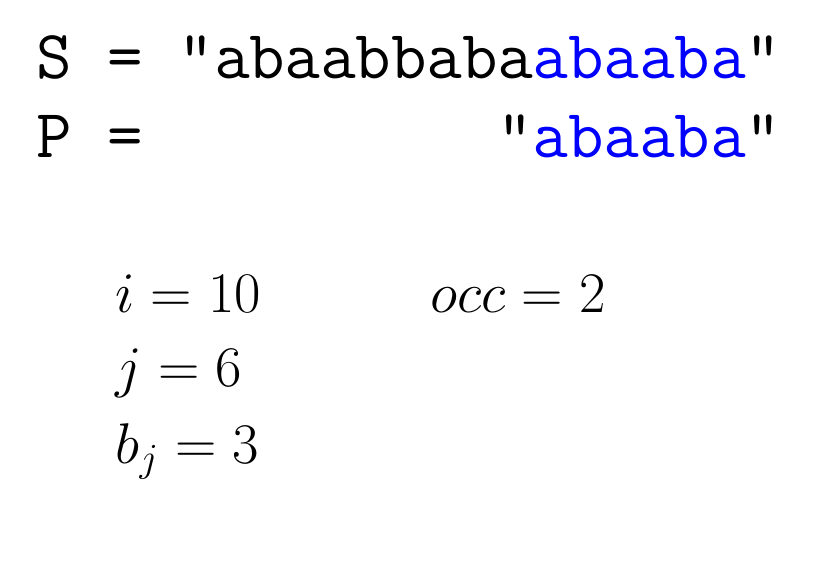
\begin{tikzpicture}
            \node[anchor=west] at (6, 5) { \Huge \texttt{S = "abaabbaba\textcolor{blue}{abaaba}\textcolor{red}{}"} };
            \node[anchor=west] at (6, 4) { \Huge \texttt{P = \ \ \ \ \ \ \ \ \ "\textcolor{blue}{abaaba}"} };

            \node[anchor=west] at (7, 2) { \huge $i = 10$ };
            \node[anchor=west] at (11, 2) { \huge $occ = 2$ };
            \node[anchor=west] at (7, 1) { \huge $j = 6$ };
            \node[anchor=west] at (7, 0) { \huge $b_j = 3$ };
            \node[opacity=0,anchor=west] at (7, -1) { \huge $s = 3$ };
        \end{tikzpicture}

    \end{figure}

\end{frame}
